\section{Thermodynamik}
\subsection{Die Zustandsgrößen}
\subsection{0. Hauptsatz der Thermodynamik}
\subsection{1. Hauptsatz der Thermodynamik}
\subsection{2. Hauptsatz der Thermodynamik}
\subsubsection{Äquivalente Formulierung des 2. Hauptsatzes}
\paragraph{Folgerungen}
\subsubsection{Die Temperatur}
\paragraph{Eichung}
\subsubsection{Die Wärme(menge)}
\subsubsection{Der Druck}
\subsubsection{Das chemische Potential}
\subsubsection{Fundamentale Gleichung}
\subsubsection{Anwendungsbeispiele}
\begin{enumerate}
  \item Entropie des idealen Gases (einatomig)
  \item Gleichheit der absoluten Temperatur $T$ und der Temperatur des idealen Gases $T_G$
  \item \emph{Wirkungsgrad} einer Wärmekraftmaschine
  \begin{figure}[H]
\begin{center}
  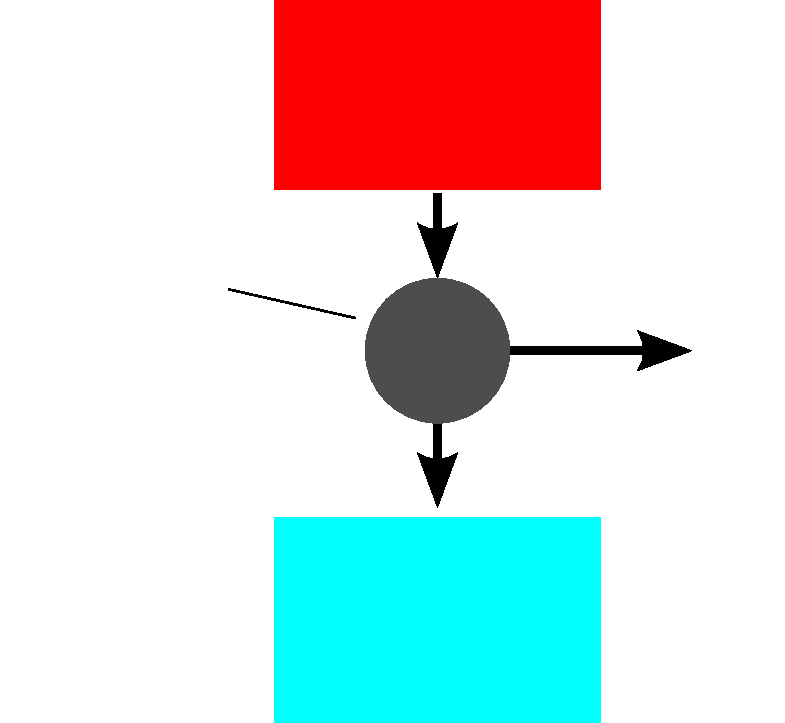
\includegraphics[width=0.3\textwidth]{../img/waermekraftmaschine.pdf}
  \caption{Wärmekraftmaschine}
  \label{img:waermekraftmaschine}
\end{center}
\end{figure}

\begin{figure}[H]
\begin{center}
  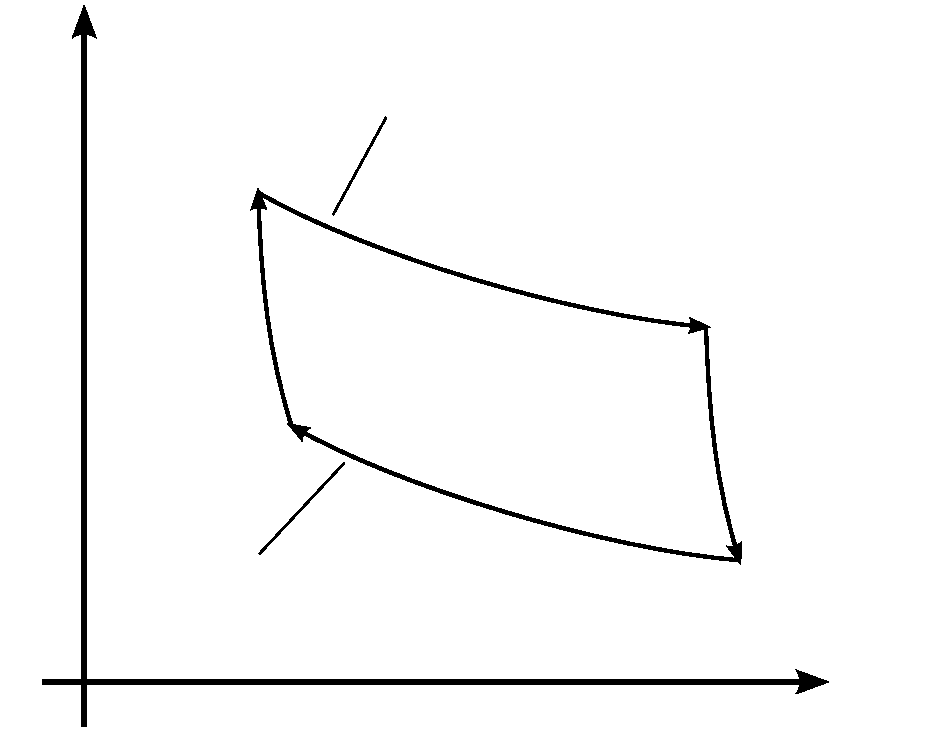
\includegraphics[width=0.3\textwidth]{../img/carnotprocess.pdf}
  \caption{Carnot-Prozess}
  \label{img:carnot}
\end{center}
\end{figure}

Reversibel:
\begin{equation}
\begin{split}
  & \Delta S = 0 \Rightarrow - \frac{Q_2}{T_2} + \frac{Q_1}{T_1} + 0  \\
  & \Rightarrow \frac{Q_2}{T_2} = \frac{Q_1}{T_1} = \gamma
\end{split}
\end{equation}
Energieerhaltung (Maschine soll nach \emph{Zyklus} im Ausgangszustan sein $\Rightarrow A = Q_2 - Q_1$) \
Wirkungsgrad $\eta$
\begin{equation}
  \eta := \frac{A}{Q_2} \Rightarrow \eta_{\text{reversibel}} = \frac{Q_2 - Q_1}{q_2} = \frac{T_2 - T_1}{T_2}
\end{equation}
Wärmepumpe:
\begin{equation}
\bar{\eta} = \frac{Q_1}{A} (\text{für } T_1 > T_2) \Rightarrow \bar{\eta}_{\text{reversibel}} = \frac{T_1}{T_1 - T_2}
\end{equation}
Kühlmaschine
\begin{equation}
\bar{\bar{\eta}} = \frac{Q_2}{-A} (\text{für } T_1 > T_2) \Rightarrow \bar{\bar{\eta}}_{\text{reversibel}} = \frac{T_2}{T_1-T_2}
\end{equation}
irreversibel:
\begin{equation}
  \Delta S > 0 \Rightarrow \frac{Q_1'}{T_1} > \frac{Q_2'}{T_2}
\end{equation}
Wirkungsgrad der Wärmekraftmaschine $\eta_{\text{irrev.}} = \frac{A'}{Q_2'}$ \\
Sei z.B. $Q_2' = Q_2 \Rightarrow Q_1' > Q_1$
\begin{equation}
\begin{split}
  \Rightarrow & A' = Q_2' - Q_1' = Q_2 - Q_1' < A \\
  \Rightarrow & \eta_\text{irrev.} < \eta_\text{reversibel}
\end{split}
\end{equation}
Wirkungsgrad der idealen \emph{Carnot-Maschine} ist maximal.
\end{enumerate}

\subsection{Einige Folgerungen aus den Hauptsätzen}
\subsubsection{Wichtige abgeleitete Größen}
\begin{itemize}
  \item Spezifische Wärme
    \begin{equation}
  	\begin{split}
  	  c_p &= \left( \frac{\Delta Q}{\Delta T} \right)_p = T \left( \frac{\partial S}{\partial T} \right)_p \\
  	  c_V &= \left( \frac{\Delta Q}{\Delta T} \right)_p = T \left( \frac{\partial S}{\partial T} \right)_V
  	\end{split}
    \end{equation}
    Technische Definition bezogen auf 1 Mol, $N=N_A$ (Avogadro) \\
    Korrekterweise: $s = \frac{S N_A}{N}, \quad v = \frac{V N_A}{N}$, siehe Adam + Hittmair \\
    hier sehen wir davon ab
  \item Kompressibilität
    \begin{equation}
   	\begin{split}
  	  \kappa_s &= - \frac{1}{V} \left( \frac{\partial V}{\partial p} \right)_S \text{ (adiabatisch)} \\
  	  \kappa_T &= - \frac{1}{V} \left( \frac{\partial V}{\partial p} \right)_T \text{ (isoterm)}
    \end{split}
	\end{equation}
  \item Ausdehungskoeffizient
  \begin{equation}
  	\alpha = \frac{1}{V} \left( \frac{\partial V}{\partial T} \right)_p
  \end{equation}
  \item Magnetische Suszeptibilität
  \begin{equation}
  	\chi = \left( \frac{\partial M}{\partial H} \right)_T
  \end{equation}
\end{itemize}
Diese Größen sind der Messung direkt zugänglich. Man beachte: die verschiedenen Größen sind nicht unabhängig, z.B. gilt 
$c_p - c_v = V T \alpha^2 / \kappa_T$ (Beweis später).
Woher kommen diese Abhängigkeiten? \emph{Integrabilitätsbeziehungen}!
\subsubsection{Maxwell-Beziehungen}
Fundamentale Gleichung \eqref{eq:fundamentalEQ}:
\begin{equation}
  \difd E = T \difd S - p \difd V + \mu \difd N, \quad E=E(S, V, N)
\end{equation}
\paragraph{Freie Energie} $F:=E - TS$ (\textsc{Legendre}-Transformation)
\begin{equation}
\begin{split}
  \Rightarrow & \difd F = \difd E - T \difd S - S \difd T \\
  \Rightarrow & \difd F = -S\difd T - p \difd V + \mu \difd N \\
  \Rightarrow & F=F(T, V, N)
\end{split}
\end{equation}
\paragraph{Enthalpie} $H:=E+pV$
\begin{equation}
\begin{split}
  \Rightarrow & \difd H = \difd E + p \difd V + V \difd p \\
  \Rightarrow & \difd H = T \difd S + V \difd p + \mu \difd N \\
  \Rightarrow & H=H(S, p, N)
\end{split}
\end{equation}
\paragraph{Freie Enthalpie} $G:=E-T+pV$
\begin{equation}
\begin{split}
  \Rightarrow & \difd G = - S \difd T + V \difd p + \mu \difd N \\
  \Rightarrow & G=G(T, p, N)
\end{split}
\end{equation}
$E, F, H, G$ heißen \emph{Thermodynamische Potentiale}. \\
\paragraph{Integrabilitätsbeziehungen} \mbox{}\\
aus $E$:
\begin{equation}
  \left( \frac{\partial T}{\partial V} \right)_{S, N} = \left( \frac{\partial p}{\partial S} \right)_{V, N}, \quad
  \left( \frac{\partial T}{\partial N} \right)_{S, V} = \left( \frac{\partial \mu}{\partial S} \right)_{V, N}, \quad
  - \left( \frac{\partial p}{\partial N} \right)_{S, V} = \left( \frac{\partial \mu}{\partial V} \right)_{S, N}
\end{equation}
aus $F$:
\begin{equation}
  \left( \frac{\partial S}{\partial V} \right)_{T, N} = \left( \frac{\partial p}{\partial T} \right)_{V, N}, \quad \text{usw.}
\end{equation}
aus $H$:
\begin{equation}
  \left( \frac{\partial T}{\partial p} \right)_{S, N} = \left( \frac{\partial V}{\partial S} \right)_{p, N}, \quad \text{usw.}
\end{equation}
aus $G$:
\begin{equation}
  - \left( \frac{\partial S}{\partial p} \right)_{T, N} = \left( \frac{\partial V}{\partial T} \right)_{p, N}, \quad \text{usw.}
\end{equation}
\textsc{Maxwell}-Beziehungen (insgesamt 12 Beziehungen) \\
\subsubsection{Exkurs: Variablentransformation}
Erwünscht:
\begin{equation}
  \left( \frac{\partial E}{\partial V} \right)_T \overset{?}{\rightarrow} \left( \frac{\partial E}{\partial V} \right)_p
  \text{ oder }
  \left( \frac{\partial E}{\partial V} \right)_T \overset{?}{\rightarrow} \left( \frac{\partial E}{\partial p} \right)_T
\end{equation}
Wichtig: Jacobi'sche Determinanten $f=f(x, y)$; $g=g(x, y)$ \\
Definition:
\begin{equation}
  \frac{\partial (f, g)}{\partial(x, y)} = \det 
  \begin{pmatrix}
  \frac{\partial f}{\partial x} & \frac{\partial f}{\partial y} \\
  \frac{\partial g}{\partial x} & \frac{\partial g}{\partial y} 
  \end{pmatrix}
  = \left( \frac{\partial f}{\partial x} \right) \left( \frac{\partial g}{\partial
  y} \right) - \left( \frac{\partial f}{\partial y} \right) \left( \frac{\partial g}{\partial x} \right)
\end{equation}
Rechenregeln
\begin{equation}
  \frac{\partial(f, g)}{\partial(x, y)} = -\frac{\partial(f, g)}{\partial(y, x)}; \qquad
  \frac{\partial(f, y)}{\partial(x, y)} = \frac{\partial f}{\partial x}
\end{equation}
und für $x=(u, v), y=(u, v)$
\begin{equation}
  \Rightarrow \frac{\partial(f, g)}{\partial(u, v)} = \frac{\partial(f, g)}{\partial(x, y)} \cdot \frac{\partial(x, y)}{\partial(u, v)}
\end{equation}
Beweis:
\begin{equation}
\begin{split}
   \det
  \begin{pmatrix}
    \frac{\partial f}{\partial u} & \frac{\partial f}{\partial v} \\
    \frac{\partial g}{\partial u} & \frac{\partial g}{\partial v}
  \end{pmatrix}
  &= \det \left[
  \begin{pmatrix}
    \frac{\partial f}{\partial x} & \frac{\partial f}{\partial y} \\
    \frac{\partial g}{\partial x} & \frac{\partial g}{\partial y}
  \end{pmatrix}
  \cdot
  \begin{pmatrix}
    \frac{\partial x}{\partial u} & \frac{\partial x}{\partial v} \\
    \frac{\partial y}{\partial u} & \frac{\partial y}{\partial v}
  \end{pmatrix}
  \right] \\
  &= \det 
    \begin{pmatrix}
    \frac{\partial f}{\partial x} & \frac{\partial f}{\partial y} \\
    \frac{\partial g}{\partial x} & \frac{\partial g}{\partial y}
  \end{pmatrix}
  \cdot \det
  \begin{pmatrix}
    \frac{\partial x}{\partial u} & \frac{\partial x}{\partial v} \\
    \frac{\partial y}{\partial u} & \frac{\partial y}{\partial v}
  \end{pmatrix} \qquad \square
\end{split}
\end{equation}
Spezialfall der Kettenregel 
\begin{equation}
  \frac{\partial(f, g)}{\partial(x, y)} \cdot \frac{\partial(x, y)}{\partial(f, g)} = 1
\end{equation}
\subsubsection{Anwendungsbeispiele} $N$ = konstant
\begin{enumerate}  % a), b)
  \item
  \begin{equation}
  \begin{split}
    c_p &=  T \left( \frac{\partial S}{\partial T} \right)_p = T \frac{\partial(S, p)}{\partial(T, p)} \overset{\text{$V$ abh.}}{=}
    T \frac{\partial(S, p)}{\partial(T, V)} / \underbrace{\frac{\partial(T, p)}{\partial(T, V)}}_{ \left( \frac{\partial p}{\partial V} \right)_T} \\ 
    &= \frac{T}{ \left( \frac{\partial p}{\partial V} \right)_T} \left[ \left( \frac{\partial S}{\partial T} \right)_V 
    \left( \frac{\partial p}{\partial V} \right) - \left( \frac{\partial S}{\partial V} \right)_T \left( \frac{\partial p}{\partial T} \right)_V \right] \\
    &= c_V - T \left( \frac{\partial S}{\partial V} \right)_T \left( \frac{\partial p}{\partial T} \right)_V / \left( \frac{\partial p}{\partial V} \right)_T \\
    &\overset{\text{Maxwell-Bez.}}{=} c_V - T \left( \frac{\partial p}{\partial T} \right)_V^2 / \left( \frac{\partial p}{\partial V} \right)_T
  \end{split}
  \end{equation}
  Nun ist
  \begin{equation}
  \begin{split}
    \left( \frac{\partial p}{\partial T} \right)_V &= \frac{\partial(p, V)}{\partial (T, V)} \\
     &= \frac{\partial (p, V)}{\partial (p, T)} \cdot \frac{\partial(p, T)}{\partial(T, V)} \\
     &= \left( \frac{\partial V}{\partial T} \right)_p \cdot \left[ - \left( \frac{\partial p}{\partial V} \right)_T \right]
  \end{split}
  \end{equation}
  \begin{equation}
    \Rightarrow c_p = c_V - T \left( \frac{\partial V}{\partial T} \right)_p^2 \left( \frac{\partial p}{\partial V} \right)_T = c_V + T V \alpha^2 / \kappa_T^2
  \end{equation}
  \item 
  \begin{equation}
    \frac{c_p}{c_v} = \frac{\kappa_T}{\kappa_S} \quad \text{(Übungsaufgabe)}
  \end{equation}
\end{enumerate}
\subsubsection{Die Gibbs-Duhem-Beziehung}
Fundamentalgleichung \eqref{eq:fundamentalEQ}, $E, S, V, N$ sind extensive Variablen
\begin{equation}
  \difd E = T \difd S - p \difd V + \mu \difd N
\end{equation}
Somit gilt für $E=E(S, V, N)$ dass $E(\alpha S, \alpha V, \alpha N) = \alpha E(S, V, N)$ (homogene Funktion nach \textsc{Euler})
\paragraph{Eulerscher Satz über homogene Funktion} $f(x_1, \ldots, x_n)$: \\
Falls $f(\alpha x_1, \ldots, \alpha x_n) = \alpha^r f(x_1, \ldots, x_n)$ so ist
\begin{equation}
  \sum_{i=1}^{n} x_i \frac{\partial f}{\partial x_i} = r f
\end{equation}
Beweis: Differentiation nach $\alpha$ und dann $\alpha = 1$ setzten. 
\paragraph{}\mbox{}\\
Damit folgt 
\begin{equation}
\begin{split}
  E &= \left( \frac{\partial E}{\partial S} \right)_{V, N} S + \left( \frac{\partial E}{\partial V} \right)_{S, N} V + \left( \frac{\partial E}{\partial N} \right)_{V, S} N \\ 
  &= T S - p V + \mu N
\end{split}
\end{equation}
Damit, im Gleichgewicht
\begin{equation}
  E = T S - p V + \mu N \qquad \text{Fundamentalrelation}
\end{equation}